\chapter{LƯỢC KHẢO CƠ SỞ LÝ THUYẾT VÀ NGHIÊN CỨU TRƯỚC}
\label{Chapter2}

\section{Tổng quan về bài toán phân tích sắc thái cảm xúc}

\subsection{Cảm xúc và sắc thái tâm trạng qua lăng kính tâm lý học}
Trong cuộc sống hàng ngày, khái niệm cảm xúc (emotion) và sắc thái tâm trạng (sentiment) thường được dùng để thay thế lẫn nhau. Tuy nhiên, trong lĩnh vực tâm lý học, chúng được coi là hai khái niệm khác biệt. Trong mô hình tâm lý học nổi tiếng mà \textcite{watson1985toward} xây dựng, đã chỉ ra cảm xúc mang cấu trúc hai chiều. Dựa trên đó, cảm xúc được định nghĩa là một trạng thái tâm lý cốt lõi phát sinh tức thời, bao gồm ba thành phần cấu trúc: trải nghiệm chủ quan, phản ứng sinh lý và phản ứng hành vi. Nhà tâm lý học \textcite{ekman1992there} đã phân loại cảm xúc thành sáu nhóm cơ bản (hạnh phúc, buồn bã, tức giận, sợ hãi, ngạc nhiên, ghê tởm), và sau này được mở rộng với các trạng thái thứ cấp như hào hứng, xấu hổ, khinh thường và thẹn thùng.

Ngược lại, sắc thái tâm trạng (sentiment) là một thái độ tinh thần mang tính tổ chức cao, được bồi đắp và hình thành dựa trên nền tảng của các cảm xúc sơ cấp. Định nghĩa này nhấn mạnh rằng "sentiment" được sử dụng để truyền tải những suy nghĩ của một cá nhân bắt nguồn từ chính cảm xúc của họ. Không giống như cảm xúc, "sentiment" tiến xa hơn một bước và không bị giới hạn trong các chiều không gian tâm lý thuần túy \parencite{yue2019survey}. Theo \textcite{mcdougall2015introduction}, sắc thái tâm trạng đóng vai trò như cầu nối giữa cảm xúc cốt lõi và chuỗi hành động có chủ đích. Nói cách khác, các loại cảm xúc đa dạng đóng vai trò như những nhân tố cấu thành nên sắc thái tâm trạng tổng thể của một cá nhân đối với một sự vật, sự việc.

\subsection{Cơ sở thần kinh học của sự biểu hiện và hiện tượng suy hao cảm xúc trong văn bản}
Dựa trên cơ sở lý thuyết của các nhà tâm lý học, các nhà khoa học thần kinh đã tiến sâu vào giải mã cơ chế sinh học của quá trình hình thành và truyền đạt cảm xúc.

Khi con người tiếp nhận một kích thích từ môi trường, tín hiệu ngay lập tức được truyền qua đồi thị (Thalamus) đến hạch hạnh nhân (Amygdala) - trung tâm xử lý cảm xúc cốt lõi, đồng thời truyền đến vỏ não trước trán (Prefrontal Cortex) để phân tích nhận thức \parencite{ledoux2013emotion}. Sau đó, hệ thần kinh tự chủ (Autonomic Nervous System) phản ứng bằng cách thay đổi nhịp tim, nhịp thở, tạo ra các "cảm giác" về mặt thể chất. Kết quả của quá trình này là các hành vi biểu hiện cảm xúc ra bên ngoài thông qua nét mặt, cử chỉ hoặc ngôn ngữ.

Tuy nhiên, khi cảm xúc phức tạp này được mã hóa xuống cấp độ ngôn ngữ dưới dạng văn bản thuần túy, một lượng lớn thông tin bị triệt tiêu. Theo nguyên tắc giao tiếp nổi tiếng của Albert Mehrabian, từ ngữ (ngôn từ) chỉ chiếm khoảng 7\% khả năng truyền tải ý nghĩa cảm xúc, phần còn lại phụ thuộc vào ngữ điệu giọng nói (38\%) và ngôn ngữ cơ thể (55\%) \parencite{mehrabian1971silent}. Do đó, một văn bản chữ viết đã đánh mất đến 93\% các manh mối cảm xúc phi ngôn ngữ.

Đối với người tiếp nhận, quá trình giải mã cảm xúc cũng sẽ đi qua một chu trình thần kinh phức tạp. Tín hiệu đầu vào (đọc văn bản, nghe âm thanh, nhìn nét mặt) được xử lý thông qua hệ thống nơ-ron gương (Mirror Neuron System) trong não bộ. Các nơ-ron này kích hoạt sự "mô phỏng" tự động, ra lệnh cho cơ thể tái hiện lại trạng thái cảm giác của người phát tín hiệu. Tín hiệu mô phỏng này sau đó được chuyển đến thùy đảo (Insula) và hạch hạnh nhân để não bộ có thể thực sự "cảm nhận", từ đó phân tích và ra quyết định phân loại sắc thái tâm trạng đó là tích cực, tiêu cực hay trung tính \parencite{iacoboni2009imitation}.

\subsection{Bài toán phân tích sắc thái cảm xúc và các cấp độ phân tích}

\textbf{Phân tích sắc thái cảm xúc (Sentiment Analysis - SA)}, hay còn được gọi là khai thác ý kiến (Opinion mining), là lĩnh vực nghiên cứu chuyên sâu về các quan điểm, thái độ và cảm xúc của con người được diễn đạt thông qua ngôn ngữ văn bản \parencite{liu2010sentiment}. Về mặt kỹ thuật, tác vụ này không chỉ dừng lại ở việc nhận diện từ vựng mang tính cảm xúc, mà là một quy trình trích xuất và phân loại các thông tin mang tính chủ quan nhằm xác định chính xác thái độ của người viết hướng tới một thực thể cụ thể \parencite{liu2010sentiment}.

Trong bài toán phân tích sắc thái cảm xúc, thuật ngữ \textit{đối tượng} ($o$) thường được dùng để chỉ thực thể mục tiêu mà người viết hướng tới, chẳng hạn như sản phẩm, dịch vụ, cá nhân hoặc tổ chức. Về mặt cấu trúc, một đối tượng $o$ có thể được phân tách thành một hệ thống phân cấp bao gồm các thành phần ($T$) và các thuộc tính ($A$). Chẳng hạn, nếu xét đối tượng $o$ là một "Video", các thành phần $T$ có thể bao gồm "nội dung", "âm thanh", "diễn viên"; các thuộc tính $A$ tương ứng có thể là "độ chân thực" hay "kỹ năng diễn xuất". Và trong đó, bản thân các thành phần này cũng có thể tiếp tục chia nhỏ thành các thành phần con $T_1$ như "phân cảnh", "thông điệp truyền tải", "lời thoại",... và các thuộc tính con $A_1$ như "độ hấp dẫn", "độ sâu sắc", "tính logic",...

Dựa trên định nghĩa này, đối tượng $o$ có thể được biểu diễn dưới dạng một cấu trúc cây phân cấp $o: (T, A)$, trong đó gốc là chính đối tượng $o$, các nút trong là các thành phần và các lá đại diện cho các thuộc tính chi tiết. Mặc dù cảm xúc có thể được biểu đạt tại bất kỳ nút nào trên cây, nhưng việc khai thác trực tiếp trên cấu trúc này thường gặp khó khăn do độ phức tạp về mặt tính toán và xử lý ngôn ngữ tự nhiên.

Do vậy, để tối ưu hóa quá trình khai thác, cấu trúc cây thường được đơn giản hóa bằng phương pháp "làm phẳng" (flattening). Khi đó, tất cả các thành phần và thuộc tính được gọi chung bằng thuật ngữ \textbf{khía cạnh} (aspect) hoặc \textbf{đặc tính} (feature), ký hiệu là $f$. Dựa trên nền tảng này, một ý kiến (opinion) sẽ được mô hình hóa chính thức dưới dạng một \textit{bộ năm thành phần (quintuple)} $(o, f, so, h, t)$, trong đó:   
\begin{itemize}
\item $o$: Đối tượng mục tiêu biểu đạt cảm xúc hay ý kiến trong văn bản.
\item $f$: Khía cạnh của đối tượng được đánh giá.
\item $so$: Hướng cảm xúc (sentiment orientation), thường mang giá trị tích cực, tiêu cực hoặc trung tính.
\item $h$: Chủ thể (holder) diễn đạt cảm xúc.
\item $t$: Thời điểm cảm xúc được biểu đạt.
\end{itemize} 
Và đối với một văn bản $d = \langle s_1, s_2, \dots, s_m \rangle$, trong đó $s_i$ là các câu cấu thành, mục tiêu của việc phân tích cảm xúc được phân định rõ ràng qua ba cấp độ nghiên cứu chính:
\begin{itemize}
    \item \textbf{Cấp độ văn bản (Document-level):} Xác định hướng cảm xúc tổng thể của toàn bộ văn bản $d$ đối với đối tượng $o$, thường được biểu diễn bằng cặp $(o, so)$.
    \item \textbf{Cấp độ câu (Sentence-level):} Xác định cảm xúc của từng câu $s_i$ đối với đối tượng $o$. Cấp độ này thường đi kèm với nhiệm vụ phân loại tính chủ quan (subjectivity classification) để phân tách câu chứa ý kiến và câu nêu sự thật.
    \item \textbf{Cấp độ khía cạnh (Aspect-level):} Xác định hướng cảm xúc đối với từng khía cạnh cụ thể $f_j$ của đối tượng $o$ được đề cập trong câu $s_i$, biểu diễn bằng bộ $(s_i, f_j, so)$. Đây là cấp độ chi tiết nhất, cho phép xử lý các văn bản chứa nhiều ý kiến phức tạp và trái ngược nhau.
\end{itemize}

\subsection{Phân tích sắc thái cảm xúc trên nền tảng học máy}

Như đã lập luận ở phần cơ sở thần kinh học, quá trình chuyển hóa cảm xúc thành văn bản thuần túy gây ra hiện tượng suy hao thông tin nghiêm trọng (lên đến 93\% các manh mối phi ngôn ngữ). Khi con người đọc văn bản, hệ thống nơ-ron gương (Mirror Neuron System) trong não bộ phải hoạt động liên tục để "mô phỏng" và bù đắp lượng thông tin khuyết thiếu này. Tuy nhiên, đối với máy tính, các phương pháp phân tích văn bản truyền thống dựa trên luật (rule-based) hoặc từ điển (lexicon) hoàn toàn bất lực trong việc khôi phục các tín hiệu cảm xúc ẩn, bởi chúng chỉ phân tích bề mặt từ vựng mà bỏ qua ngữ cảnh và cấu trúc ngữ nghĩa sâu xa \parencite{liu2012sentiment}.

Để giải quyết thách thức này, các phương pháp tiếp cận dựa trên Học máy (Machine Learning) và Học sâu (Deep Learning) ra đời, đóng vai trò như một "hệ thống nơ-ron gương kỹ thuật số". Thay vì dựa vào các quy tắc cứng nhắc, các thuật toán học máy có khả năng tự động trích xuất các biểu diễn đặc trưng phi tuyến tính (non-linear representations) từ các tập dữ liệu lớn. Thông qua việc phân tích tần suất xuất hiện, vị trí, và mối liên kết ngữ cảnh giữa các từ, hệ thống có thể học cách suy luận và dự đoán sắc thái tâm trạng một cách tự động và chính xác.

Sự phát triển của phân tích sắc thái cảm xúc trên nền tảng học máy trải qua các giai đoạn chính:
\begin{itemize}
    \item \textbf{Học máy truyền thống (Traditional Machine Learning):} Các thuật toán như Support Vector Machine (SVM), Naive Bayes, hay Logistic Regression sử dụng các kỹ thuật trích xuất đặc trưng thủ công như Bag-of-Words (BoW) hoặc TF-IDF. Mặc dù mang lại hiệu quả cao hơn phương pháp từ điển, nhóm này vẫn gặp hạn chế lớn trong việc hiểu chuỗi ngữ cảnh dài và thứ tự từ vựng.
    \item \textbf{Học sâu (Deep Learning):} Sự ra đời của các Mạng nơ-ron nhân tạo (Artificial Neural Networks) như RNN, CNN, LSTM và đặc biệt là kiến trúc Transformer đã tạo ra bước đột phá. Các mô hình này có khả năng nhúng từ vựng vào một không gian véc-tơ đa chiều (Word Embeddings), giúp biểu diễn trọn vẹn mối quan hệ ngữ nghĩa tinh vi và tự động phân tách đối tượng $o$ cùng khía cạnh $f$ trong bộ năm thành phần $(o, f, so, h, t)$.
\end{itemize}

Về mặt định nghĩa toán học, quá trình phân tích sắc thái cảm xúc bằng học máy là việc xấp xỉ một hàm mục tiêu để ánh xạ từ không gian văn bản đầu vào sang không gian nhãn cảm xúc. Gọi $\mathcal{D} = \{d_1, d_2, \dots, d_n\}$ là tập hợp các văn bản (hoặc câu, bình luận) cần phân tích. Gọi $\mathcal{E}$ là không gian nhãn cảm xúc được định nghĩa trước (ví dụ: $\mathcal{E} = \{Tích\ cực, Tiêu\ cực, Trung\ tính\}$ đối với phân loại 3 cực).

\subsection{Tổng quan về các thách thức phân tích sắc thái cảm xúc trên nền tảng YouTube}

\section{Tổng quan về phương pháp luận - Methodological Framework}
Hiện nay, cộng đồng học thuật vẫn chưa có một định nghĩa chính thức về \textbf{khung phương pháp luận (methodological framework)}. Tuy nhiên, có một sự đồng thuận ngầm rằng đây là một công cụ giúp dẫn dắt người thực hiện đi qua một chuỗi các bước có trình tự để hoàn thành một quy trình cụ thể. Trong đó, \textbf{phương pháp luận} được hiểu là tập hợp các phương pháp trong một lĩnh vực chuyên biệt, còn \textbf{khung} đóng vai trò là cấu trúc của các quy tắc hoặc ý tưởng nền tảng. Việc áp dụng khung phương pháp luận không chỉ giúp cải thiện tính nhất quán, tính chặt chẽ mà còn chuẩn hóa các cách tiếp cận, từ đó tối đa hóa độ tin cậy của các kết quả nghiên cứu \parencite{mcmeekin2020methodological}.

Dựa trên các tiền đề đó, một khung phương pháp luận chất lượng cần đáp ứng các tiêu chí cốt lõi sau.

    \begin{itemize}
        \item \textbf{Tính hệ thống (Systematicity)}: Các bước phải được sắp xếp theo trình tự logic, có sự liên kết chặt chẽ và nhất quán xuyên suốt quy trình.
        \item \textbf{Tính toàn diện (Comprehensiveness)}: Bao quát đầy đủ các giai đoạn cần thiết, từ khâu xác định bằng chứng đến khâu thực thi và đánh giá.
        \item \textbf{Tính linh hoạt (Flexibility)}: Có khả năng điều chỉnh và thích nghi với các bối cảnh nghiên cứu khác nhau mà không phá vỡ cấu trúc cốt lõi.
        \item \textbf{Tính khả thi và Thực chứng (Feasibility \& Evidence-based)}: Khung phải được xây dựng dựa trên dữ liệu thực tế, kinh nghiệm chuyên gia và có khả năng ứng dụng thực tiễn cao thông qua việc thử nghiệm (pilot).
    \end{itemize}

    Với phạm vi đề tài, trong các nghiên cứu gần đây về xây dựng khung phương pháp cho bài toán phân tích cảm xúc (Sentiment Analysis), dù thực hiện trên dữ liệu tiếng Việt hay các ngôn ngữ khác, quy trình thực hiện đa phần đều tuân thủ các giai đoạn chuẩn hóa bao gồm: thu thập dữ liệu, tiền xử lý, tách từ (tokenization) và vector hóa, huấn luyện mô hình, và cuối cùng là đánh giá, biểu diễn kết quả (\cite{el2025transformer}, \cite{singh2021youtube}). Quy trình hệ thống này cũng tương đồng với khung phương pháp luận do Uma Maheswari cùng các cộng sự đề xuất (Hình \ref{fig:sa_framework}).

    \begin{figure}[H]
        \centering
        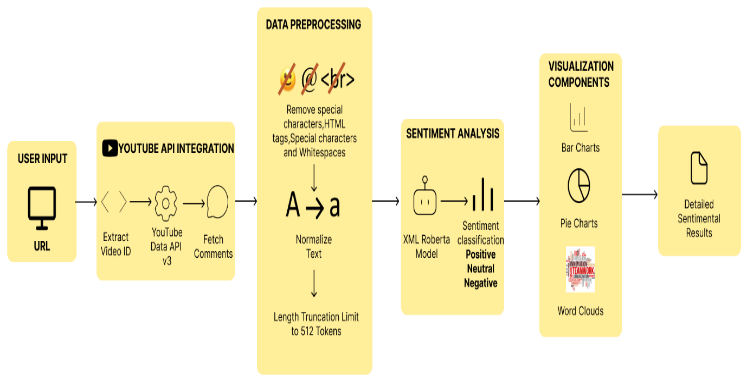
\includegraphics[width=0.8\textwidth]{Images/framework_sample.png}
        \caption{Khung phương pháp luận chung cho bài toán phân tích sắc thái cảm xúc được Uma Maheswari cùng các cộng sự đề xuất \cite{Maheswari2024Sentiment}.}
        \label{fig:sa_framework}
    \end{figure}

    Ngoài ra, khi khảo sát các công trình nghiên cứu chuyên biệt về văn bản tiếng Việt cho thấy, trọng tâm hiện nay chủ yếu tập trung vào việc cải tiến cấu trúc các mô hình học máy nhằm tối ưu hóa độ chính xác (\cite{minh2024fine}, \cite{nguyen2025like}, \cite{quoc2023vietnamese}). Tuy nhiên, xu hướng này dẫn đến việc ưu tiên quá mức các chỉ số định lượng (như Accuracy, F1-score) trên các bộ dữ liệu mẫu (benchmark datasets) mà chưa chú trọng đúng mức đến việc xây dựng một quy trình xử lý chuẩn hóa có tính thích ứng cao. Hệ quả là các mô hình thường đạt hiệu suất tối ưu trong môi trường thực nghiệm nhưng lại bộc lộ hạn chế về tính linh hoạt khi triển khai trên dữ liệu thực tế — nơi ngôn ngữ biến đổi liên tục và có độ nhiễu cao như các bình luận trên nền tảng YouTube.

\section{Tổng quan về các mô hình dựa trên Transformer}

\textbf{Kiến trúc Transformer}, được giới thiệu bởi Vaswani và các cộng sự \cite{vaswani2017attention}, đã tạo nên một bước ngoặt quan trọng trong lĩnh vực xử lý ngôn ngữ tự nhiên (NLP). Mà trọng tâm của kiến trúc này là cơ chế tự chú ý (Self-Attention) (Hình \ref{fig:attetion}), cho phép mô hình tính toán mối quan hệ giữa các từ trong một chuỗi văn bản một cách hiệu quả, bất kể khoảng cách giữa chúng.

    Về mặt cấu trúc, Transformer bao gồm hai thành phần cốt lõi, bộ mã hóa (Encoder) và bộ giải mã (Decoder) (Hình \ref{fig:transformer}), được xếp chồng lên nhau thành nhiều lớp. Trong đó:
    
    \begin{itemize}
        \item \textbf{Bộ mã hóa}: Đảm nhận việc xử lý dữ liệu đầu vào để tạo ra các biểu diễn ngữ nghĩa (embeddings) đa chiều và phong phú.
        \item \textbf{Bộ giải mã}: Khai thác các biểu diễn này để sinh ra chuỗi đầu ra mục tiêu.
    \end{itemize}
    
    Đồng thời, cơ chế tự chú ý cũng đóng vai trò quyết định giúp mô hình tập trung vào các thành phần quan trọng trong văn bản, từ đó tối ưu hóa khả năng hiểu ngữ cảnh và các liên kết ngữ nghĩa phức tạp. Mà dựa trên nền tảng này, các nghiên cứu sau đó cũng đã phát triển thành các nhánh mô hình chủ đạo.
    
    \begin{itemize}
        \item \textbf{Họ mô hình chỉ có bộ mã hóa (Encoder-only)}: Điển hình là BERT \cite{devlin2019bert} và RoBERTa \cite{liu2019roberta}. Nhóm này tập trung vào việc trích xuất đặc trưng ngữ nghĩa sâu sắc, phục vụ các tác vụ như phân loại văn bản, trích xuất thông tin và phân tích cảm xúc.

        \item \textbf{Họ mô hình chỉ có bộ giải mã (Decoder-only)}: Tiêu biểu là dòng GPT \cite{radford2018improving}, được tối ưu hóa cho việc sinh văn bản tự nhiên, hỗ trợ hiệu quả các nhiệm vụ như trả lời câu hỏi, tóm tắt và sáng tạo nội dung.
    \end{itemize}

    Và hiện nay, hầu hết các nghiên cứu tiên tiến về phân tích sắc thái cảm xúc đều kế thừa sức mạnh từ các kiến trúc dựa trên Transformer nhằm đạt được hiệu suất tối ưu (\cite{minh2024fine}, \cite{nguyen2025like}, \cite{quoc2023vietnamese}).
    
    \begin{figure}[H]
        \centering
        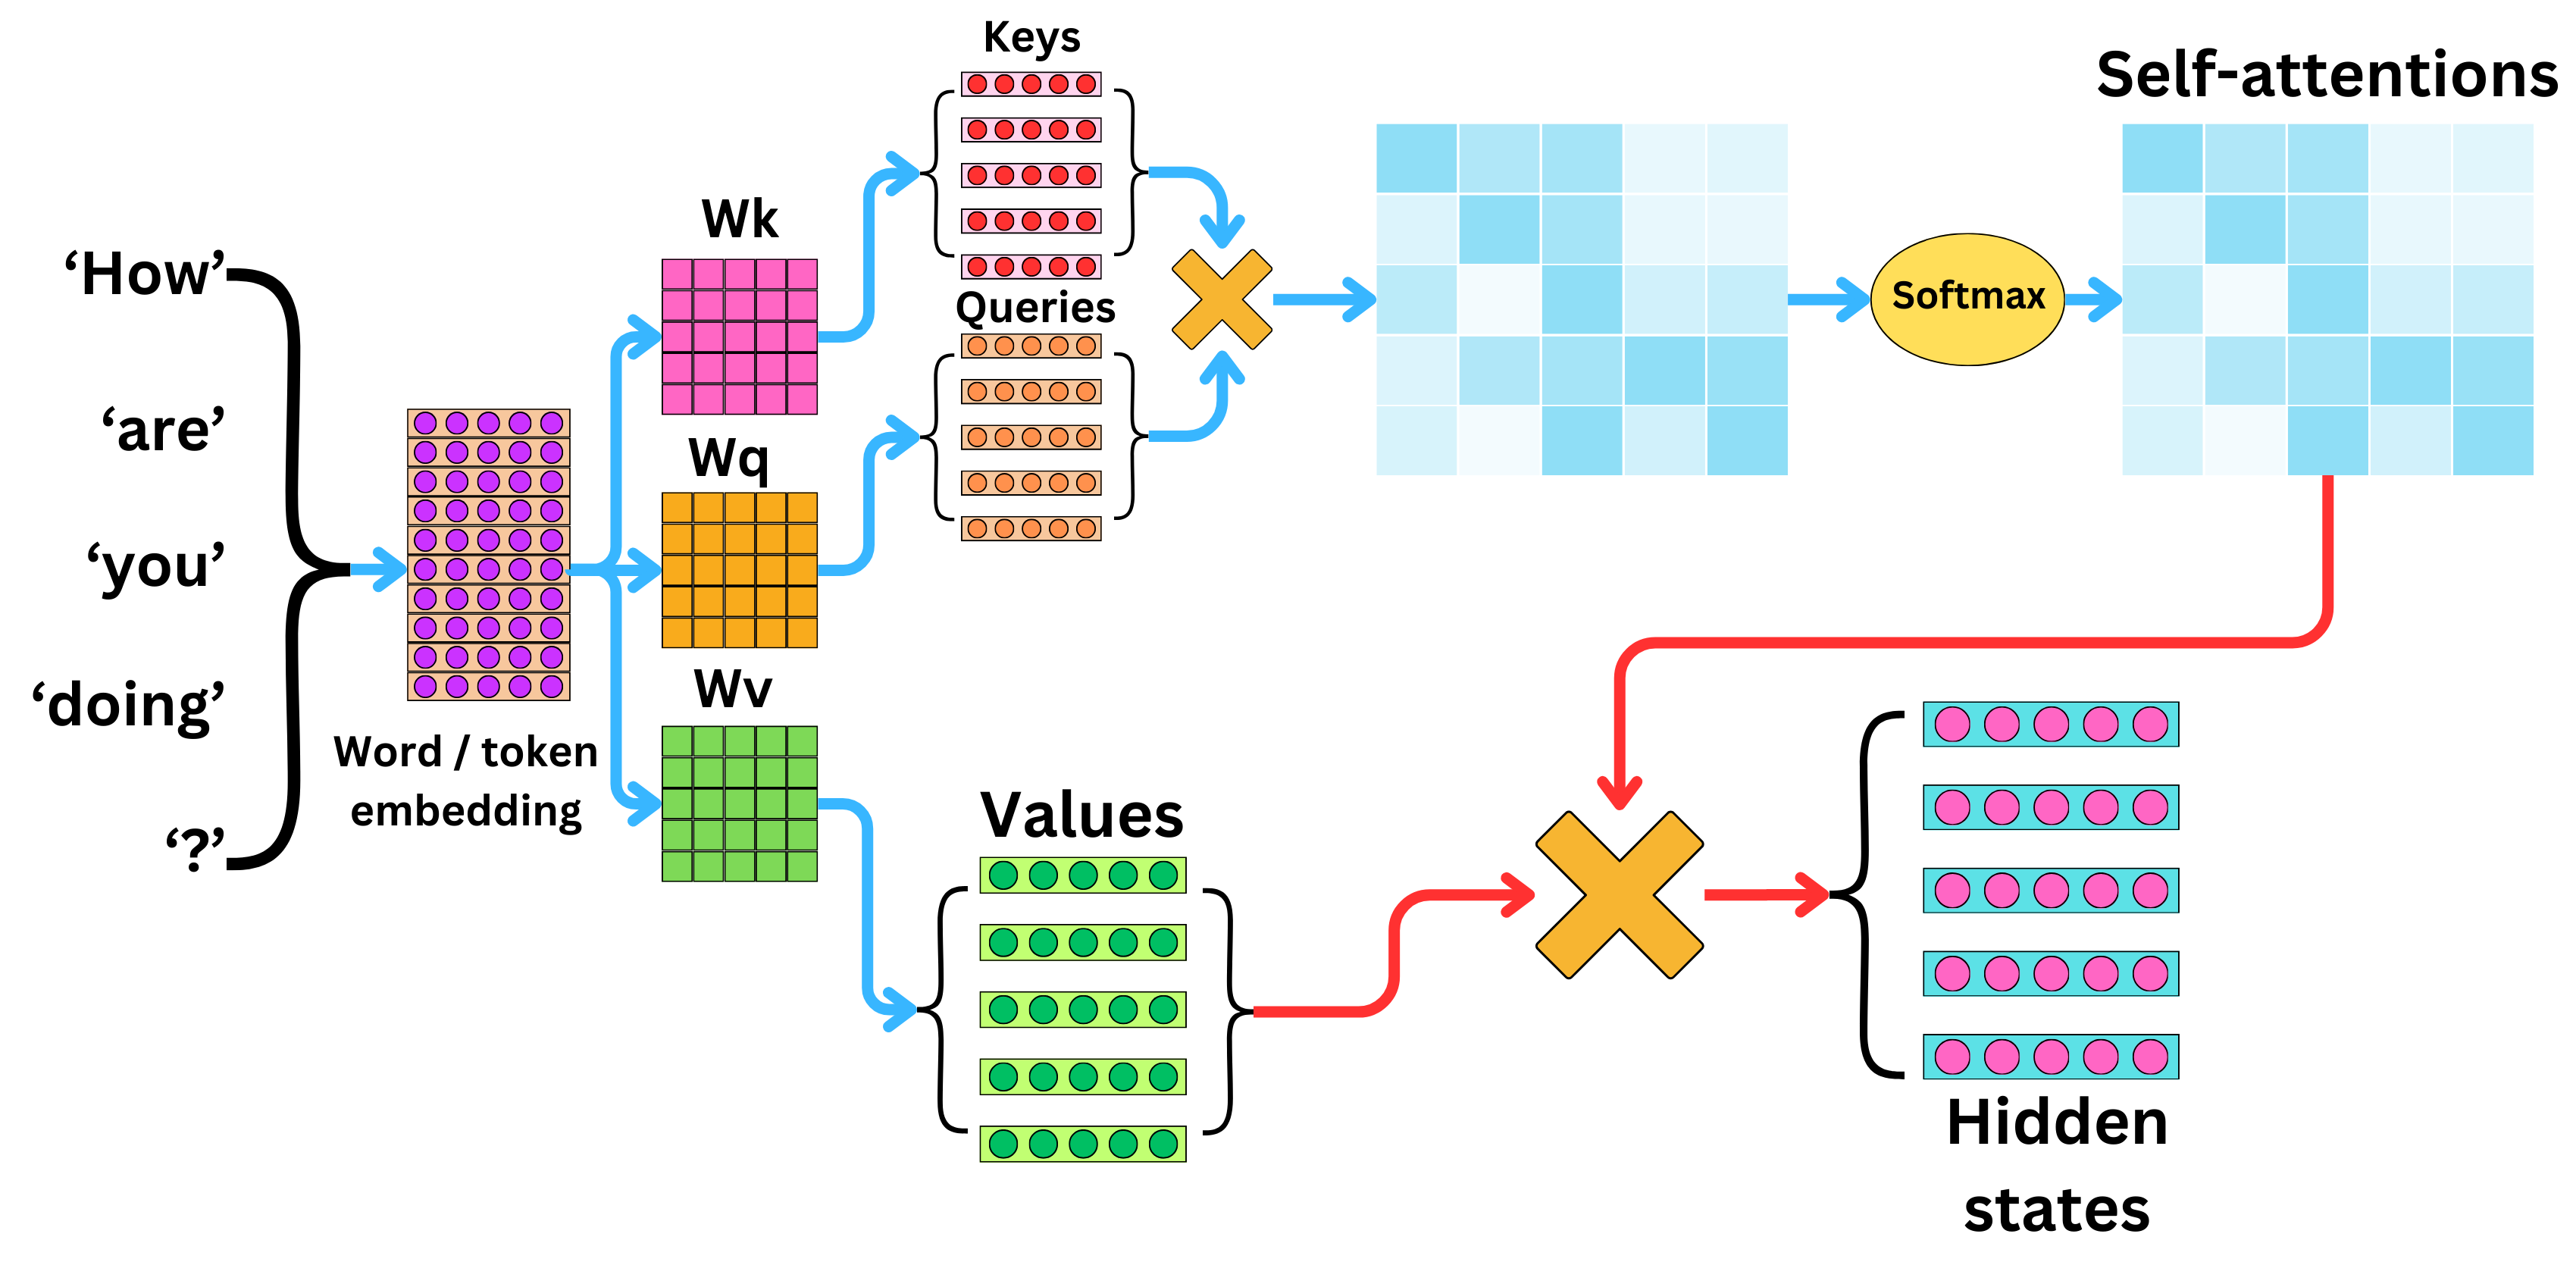
\includegraphics[width=0.8\textwidth]{Images/attention.png}
        \caption{Kiến trúc cơ chế tự chú ý (Self-Attention) trong Transformer \cite{vaswani2017attention}.}
        \label{fig:attetion}
    \end{figure}

    \begin{figure}[H]
        \centering
        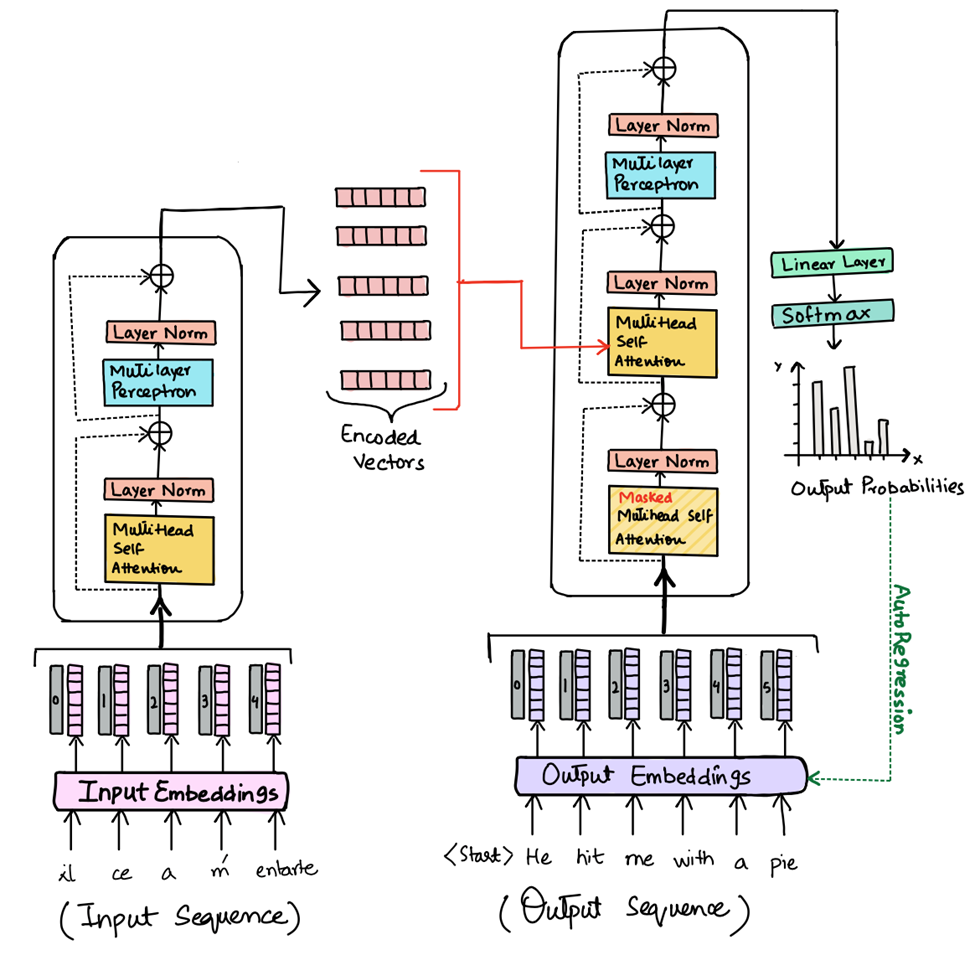
\includegraphics[width=0.8\textwidth]{Images/transformer.png}
        \caption{Kiến trúc tổng thể của Transformer với các lớp Encoder và Decoder \cite{vaswani2017attention}.}
        \label{fig:transformer}
    \end{figure}

\section{Các nghiên cứu liên quan}

\subsection{Tình hình nghiên cứu ngoài nước}
Trên thế giới, bài toán phân tích sắc thái cảm xúc đối với các ngôn ngữ phổ biến đã đạt được rất nhiều thành tựu đáng kể. Phần lớn các nghiên cứu tiên tiến nhất hiện nay đều đã chuyển dịch sang việc áp dụng các mô hình học máy dựa trên kiến trúc Transformer để giải quyết hiệu quả các bài toán phân tích đa miền (multi-domain). Bên cạnh việc tối ưu độ chính xác của mô hình, các nghiên cứu quốc tế cũng đã đề xuất và áp dụng thành công các khung phương pháp luận hệ thống chuyên biệt để xử lý dữ liệu mạng xã hội, bao gồm các bước chuẩn hóa từ việc trích xuất API, tiền xử lý văn bản nhiễu cho đến trực quan hóa kết quả đầu ra.

\subsection{Tình hình nghiên cứu trong nước}
Tại Việt Nam, mặc dù tiếng Việt thuộc nhóm 20 ngôn ngữ có quy mô cộng đồng sử dụng lớn nhất thế giới, các nghiên cứu về phân tích cảm xúc hiện nay phần lớn vẫn chỉ tập trung vào các tập dữ liệu ngách thuộc một miền (domain) cụ thể. Trọng tâm của các công trình nghiên cứu chuyên biệt về văn bản tiếng Việt chủ yếu tập trung vào việc cải tiến cấu trúc các mô hình học máy để tối ưu hóa các chỉ số định lượng (như Accuracy, F1-score) trên các bộ dữ liệu mẫu (benchmark datasets).

Tuy nhiên, xu hướng này dẫn đến một hạn chế lớn là chưa chú trọng đúng mức đến việc xây dựng một quy trình xử lý chuẩn hóa có tính thích ứng cao. Hệ quả là các mô hình thường đạt hiệu suất tốt trong môi trường thực nghiệm nhưng lại bộc lộ nhiều điểm yếu về tính linh hoạt khi triển khai trên dữ liệu thực tế – nơi ngôn ngữ biến đổi liên tục và có độ nhiễu cao như bình luận trên YouTube. Ngoài ra, tiếng Việt còn đối mặt với nhiều thách thức đặc thù về ngôn ngữ chưa được giải quyết triệt để như sự khác biệt phương ngữ, hiện tượng trộn mã (code-switching), hệ thống từ Hán - Việt mang sắc thái tu từ riêng, và sự thiếu phân biệt thị giác giữa các từ đồng âm khác nghĩa do đặc trưng của chữ Quốc ngữ.

\subsection{Tổng hợp và nhận định nghiên cứu}
